\documentclass{beamer}

\usepackage[utf8]{inputenc}
\usepackage[T1]{fontenc}
\usepackage[francais]{babel}

\usetheme{Darmstadt}
\usecolortheme{seahorse}

\usepackage{graphicx}
\input{/home/pablo/Documents/Examples/lstset}

\AtBeginSection[]{
    \begin{frame}
        \frametitle{Plan}
        \tableofcontents[currentsection,hideothersubsections]
    \end{frame} 
}

\title{Projet TopSolid}
\author{Ariane Lefebvre \and Sina Miladi \and Pablo Coves}
\date{}

\begin{document}
\maketitle

\section{Description du projet}
\subsection{TopSolid}
\begin{frame}
    \begin{columns}
        \column{.5\textwidth}
        Description de l'entreprise.
        \column{.5\textwidth}
        \begin{figure}
            
\includegraphics[width=\textwidth]{img/topSolid.jpg}
            \caption{TopSolid Galaxy}
            \label{TopSolid}
        \end{figure}
    \end{columns}
\end{frame}
\subsection{Mots clés}
\begin{frame}
    \begin{columns}
        \column{.5\textwidth}
        \frametitle{Une scène}
        Une scène est composée de plusieurs éléments:
        \begin{itemize}
            \item Une matrice:\\
                Définie par un polygone, fixe au cours du temps.
            \item Un poinçon:\\
                Défini par un polygone dont on connait le mouvement au cours du temps.
            \item Une tôle:\\
                Considérée d'épaisseur fixe, elle est décrite par sa fibre neutre.
        \end{itemize}
        \column{0.5\textwidth}
        \begin{figure}
            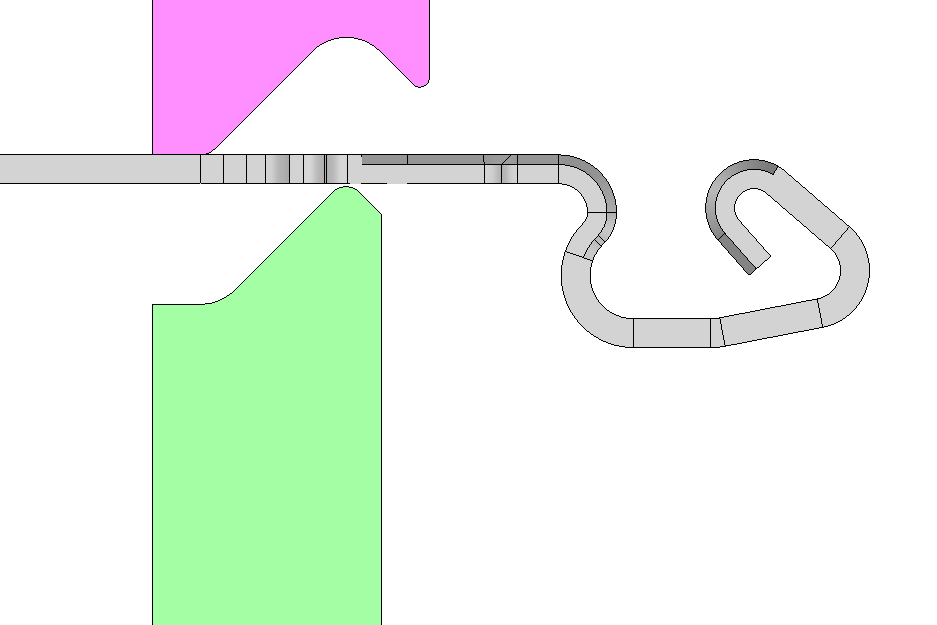
\includegraphics[width=\textwidth]{img/fibreNeutre.jpg}
            \caption{Fibre neutre}
            \label{FibreNeudre}
        \end{figure}
    \end{columns}
\end{frame}
\begin{frame}
    \frametitle{Une étape}
    \begin{columns}
        \column{.7\textwidth}
        Chaque position du poinçon correspond à une étape d'une scène.\\
        Il faut prendre en compte:
        \begin{itemize}
            \item Les forces appliquées sur la tôle.
            \item Le déplacement induit par ces forces.
            \item Le retour élastique lors du retrait du poinçon.
        \end{itemize}
        \column{.3\textwidth}
        \begin{figure}
            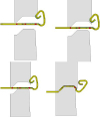
\includegraphics[width=\textwidth]{img/etape.jpg}
            \caption{Étapes}
            \label{Étape}
        \end{figure}
    \end{columns}
\end{frame}

\section{Description du logiciel}
\subsection{Freefem++}
\begin{frame}
    \frametitle{Gestion de la déformation}
    \begin{columns}
        \column{.5\textwidth}
        Un logiciel de résolution d'équations différentielles par élément finis.\\
        Il est utilisé pour:
        \begin{itemize}
            \item Générer un maillage pour la représentation.
            \item Calculer le déformation de la tôle selon les forces appliquées.
        \end{itemize}
        \column{.5\textwidth}
    \end{columns}
\end{frame}
\subsection{QGLWidget}
\subsection{Interface utilisateur}

\section{Organisation}
\subsection{Diagramme de Gantt}

\section{Conclusion}
\subsection{Avantages et défauts}
\subsection{Questions}

\end{document}
